\chapter{Introduction}
\noindent Medical imaging is an important tool in modern health care, assisting in the diagnosis, treatment planning, and monitoring of diseases.
With the advances of deep learning techniques, automated image segmentation has opened up new possibilities in terms of precision and efficiency\cite[1-2]{zhou_review_2021}.
However, as the volume and resolution of medical images increase, so does the demand for computational power\cite[1]{wang_super-resolution_2023}.
For companies and individuals with low computational resources, the challenge thus becomes: How can we maintain high-quality segmentations while still being memory-efficient?\\[1ex]
Among the myriad of deep learning architectures, the U-Net stands out in the domain of medical image segmentation.
Originally designed for biomedical image segmentation, its unique architecture allows it to incorporate both spatial and detailed high-resolution information to produce precise segmentations\cite{ronneberger_u-net_2015}.
This makes it ideal for medical image segmentation tasks where it has to differentiate between tissues and find regions of interest in an MRI scan.
However, like many deep neural networks, when it is scaled to handle large $3$D volumes, as is often the case with raw MRI scans, the GPU memory consumption can become a bottleneck.
The aim of this work is to investigate different model topology adaptations of the U-Net that try to mitigate this problem.

\section{Bachelor Project}
This research is a subset of a broader initiative aimed at constructing the Medical Image Annotation Platform (MIA), an integral component of the VISIAN editor.
The VISIAN editor is a web-based application that can be found on the \href{https://visian.org/}{VISIAN website}. Further readings on MIA can be found \href{https://mia-ai.vercel.app/}{here}.
At its core, the VISIAN frontend strives to deliver an intuitive interface tailored for healthcare professionals, simplifying the intricate process of medical image segmentation.
While the traditional manual segmentation approach proves to be labor-intensive and monotonous, the MIA backend, in synergy with VISIAN's functionalities,
introduces a `human-in-the-loop' methodology to this domain.\\[1ex]
Within this loop, medical specialists initiate the annotation of a dataset, setting the stage for training a machine learning model. While users have the flexibility to upload their models,
plans are underway to offer a curated selection of diverse models, allowing users to choose one that aligns best with their requirements. Once a model is selected, it can be trained on the initial annotations,
after which it produces segmentations for review. Medical professionals can then examine, refine, and amend these segmentations.
This iterative process continues until the segmentations achieve the desired level of accuracy and precision. A defining strength of this system is its capability to streamline the segmentation process.
The machine learning model not only delivers a robust starting point but continues to provide enhanced suggestions as the cycle progresses, enabling medical experts to work with heightened efficiency.\\[1ex]
Moreover, acknowledging the sensitive nature of medical data, the platform has been architected to operate locally on the user's machine, ensuring data privacy and security.
Such a design consideration brings forth its own set of challenges, particularly in the realm of computational capabilities.
Given that many users might not have access to multiple high-end GPUs and that consumer-grade GPUs often feature limited memory capacity, there is an imperative to optimize our models for memory efficiency,
ensuring wide accessibility and functionality across diverse hardware configurations.

\section{Approaches to Decrease Memory Consumption}
Before delving into the specific adaptations we've made to the U-Net architecture, it is important to recognize the larger landscape of memory efficiency in deep learning.
Tackling the challenges of large datasets and the associated memory consumption is a widespread concern,
and various strategies, such as the following, have been proposed:
\begin{enumerate}
	\item \textbf{Model Pruning}: This technique involves removing certain neurons or weights that contribute minimally to the model's predictive power.
	Pruned models often retain their performance, or only slightly degrade, while being much more lightweight\cite{chong_resource_2023}.
	\item \textbf{Quantization}: By representing model parameters with fewer bits, quantization reduces the memory footprint of the model. Typically,
	weights in neural networks are stored as $32$-bit floats. Through quantization, these can be represented with just $8$ bits (or even less), leading to considerable memory savings\cite{gholami_survey_2021}.
	\item \textbf{Memory-efficient Backpropagation}: Traditional backpropagation in training deep networks can be memory-intensive due to the storage of intermediate values for gradient computation.
	New approaches, such as reversible backpropagation, allow for recomputation of these values, trading off computation time for memory savings\cite{brugger_partially_2019}.
\end{enumerate}
While these methods provide a comprehensive toolkit for memory efficiency, our exploration zeroes in on the model topology, specifically adaptations to the U-Net architecture.
As we'll see, adjusting the architecture can lead to notable memory efficiency increases.

\section{U-Net}
In this study, our primary aim is to refine the U-Net architecture for enhanced memory efficiency. To meticulously comprehend the modifications made to the standard U-Net,
along with their benefits and limitations, a thorough understanding of the foundational U-Net is pivotal.

\subsection{Convolutional Layers}
Within the realm of deep learning, convolutional neural networks (CNNs) have emerged as the gold standard for tasks related to computer vision.
The U-Net architecture harnesses the inherent strengths of CNNs to its advantage.\\[1ex]
\noindent At the heart of CNNs lies the `convolutional layer', a unique structure inspired by the human visual cortex designed to automatically and adaptively learn spatial hierarchies of features from images.
A convolutional layer operates using `filters' or `kernels'. These are small, learnable weight matrices that move across the input data (such as an image) to produce a feature map, or `convolved feature'.
The primary idea is that instead of connecting every neuron to every other neuron in consecutive layers (as in fully connected layers),
a convolutional layer has neurons connected to only a local region in the input, and all neurons share the same weights. This reduces the number of parameters,
allowing the network to be deeper with fewer parameters\cite[5-7]{oshea_introduction_2015}.

\begin{figure}[!hb]
	\centering
	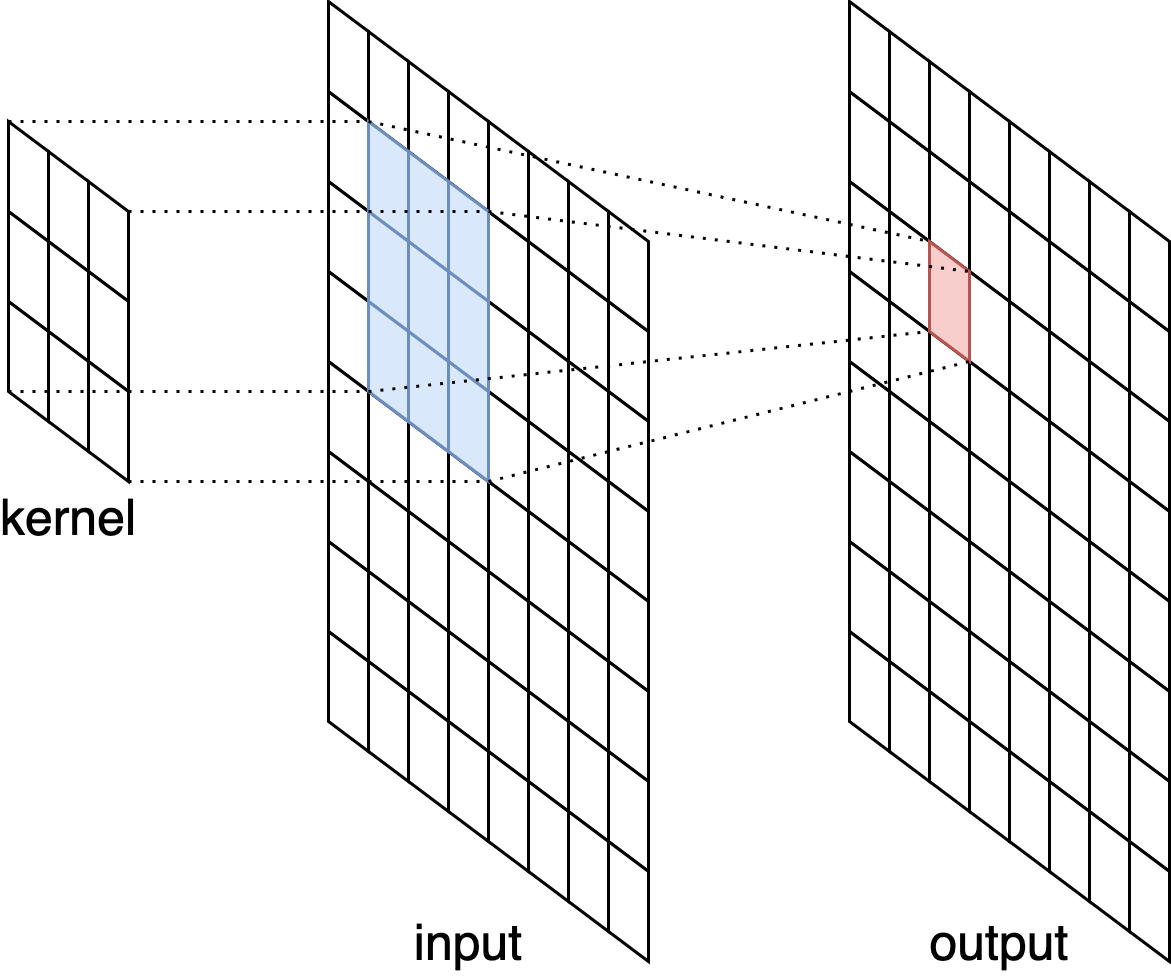
\includegraphics[width=0.4\linewidth]{images/Convolution}
	\caption{Convolutional Layer. The picture depicts a $3\times3$ kernel, that is convolved over a $5\times5$ image (input). Producing a $5\times5$ feature map (output).}
	\label{fig:Conv}
\end{figure}

\noindent This process of convolution can best be visualized as shining a flashlight over a dark image (\autoref{fig:Conv}). As the flashlight moves (or `convolves') around the image,
it illuminates different parts, and the illuminated section is transformed through the filter. The output is a new image that highlights certain features, edges, textures,
or shapes depending on what the filter is designed or has learned to detect.
The strength of convolutional layers is their ability to learn patterns with translational invariance. This means,
if a pattern is learned in one part of an image, the same pattern can be recognized in a different part without explicitly training for that location.
This property is especially advantageous for image recognition tasks where the same feature, such as the edge of an object or the texture of a surface, can appear anywhere in the image.\\[1ex]
In summary, convolutional layers form the foundational building blocks of CNNs, enabling the network to automatically learn hierarchical and spatially invariant features,
which are essential for tasks like image classification, object detection, and many other applications in the realm of computer vision.

\subsection{U-Net Architecture}
Building on the foundational principles of CNNs,
the U-Net architecture presents a specialized deep learning structure that has proven to be highly effective for tasks like biomedical image segmentation.
Originally introduced by Olaf Ronneberger, Philipp Fischer, and Thomas Brox in $2015$\cite{ronneberger_u-net_2015}, U-Net addresses challenges unique to medical imaging, such as the need for high-resolution output,
fewer training samples, and intricate structures.

\begin{figure}[!hb]
	\centering
	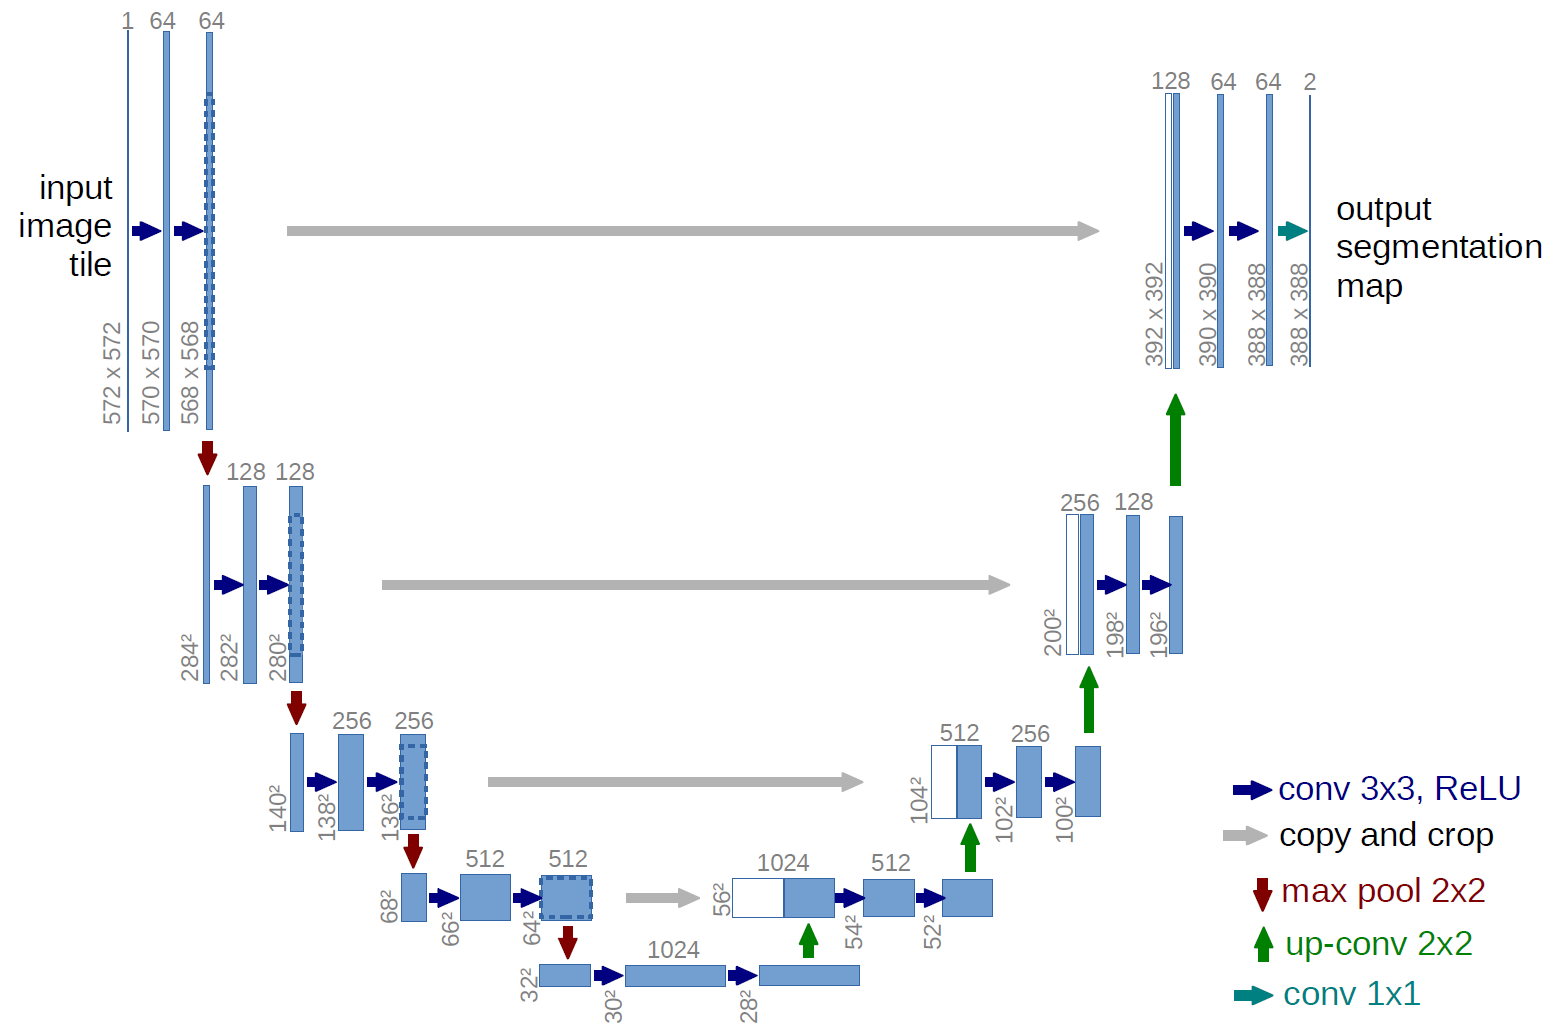
\includegraphics[width=0.8\linewidth]{images/UNet-Architecture}
	\caption{U-Net Architecture. Each blue box corresponds to a multichannel feature map.
	The number of channels is denoted on the top of the box.
	The x-y-size is provided at the lower left edge of the box.
	White boxes represent copied feature maps.
	The arrows denote the different operations\cite[2]{ronneberger_u-net_2015}.}
	\label{fig:UNet}
\end{figure}

\noindent The name `U-Net' is derived from its U-shaped architecture.
This shape essentially consists of two primary parts:\\[1ex]
\noindent\textbf{Contracting (Downsampling) Path}\\
This is the `encoder' and looks very much like a traditional CNN.
Starting with the input image, this pathway consists of a series of convolutional layers followed by max-pooling layers.
As we move deeper into the network through this path,
the spatial dimensions of the feature maps decrease, but the depth (number of channels) increases.
This captures increasingly abstract representations of the input image,
compressing the spatial information but enriching the contextual details.\\[1ex]
\noindent\textbf{Expansive (Upsampling) Path}\\
This is the `decoder' where U-Net starts to differentiate itself from other CNNs.
In this path, the spatial dimensions of the feature maps are gradually increased using up-convolutions
(or transposed convolutions). This helps recover the spatial information required for precise segmentation.
Additionally, at every step of this pathway, there's a crucial skip connection from the corresponding layer in the contracting path.
This means that the high-resolution features from the downsampling path are concatenated with the upsampled features.
Such skip connections ensure that the localization information is not lost,
which is crucial for achieving precise boundaries in segmentation tasks\cite[4]{ronneberger_u-net_2015}.\\[1ex]
The final layer of the U-Net is a convolution that maps the multichannel feature map to the desired number of classes, essentially assigning each pixel of the image to a particular segment.\\[1ex]
\textbf{Advantages and Challenges}\\
This intricate structure allows the U-Net to capture high-resolution local information in the upper parts of the U-Net and low-resolution global information in the bottom parts of the U-Net,
enabling it to come up with precise and accurate segmentations. The skip connections are particularly significant, bridging the gap between the high-resolution input and precise segmentation output.
Moreover, U-Net's efficient use of data, requiring fewer annotated images for training, is a significant advantage, especially in the domain of biomedical imaging, where labeled data can be scarce.\\[1ex]
However, every silver lining has its cloud. One of the challenges when using the U-Net architecture arises when handling high-resolution $3$D data. While U-Net excels with high-resolution $2$D images,
translating this to $3$D data dramatically increases the computational and memory demands. This is primarily due to the increase in spatial dimensions: in $3$D,
every slice of data contributes additional information that the network must process, making the memory footprint substantially larger. As a result,
processing large $3$D datasets can become particularly taxing on the GPU's memory. This limitation can make the architecture unsuitable for consumer-grade graphics cards,
hindering its widespread application in some $3$D imaging contexts.

\subsection{Patch-wise U-Net}
Given the inherent challenges posed by the U-Net architecture when managing high-resolution $3$D datasets, there emerges an essential need to develop a more adaptable and resource-efficient approach.
Enter the patch-wise U-Net.\\[1ex]
The patch-wise U-Net operates on the principle of segmenting the larger scan into small, manageable patches, allowing for individual processing of each segment\cite[5-7]{lee_automatic_2020}.
This methodology reduces the GPU's memory demands. Depending on how much the original scan is patchified, we will get a small or great memory reduction. However, with every solution comes a unique set of challenges.
By segmenting the dataset and analyzing it in patches, the neural network inherently loses the global context of the entire image.
This local view can potentially compromise the accuracy of segmentations, as the model might miss out on leveraging crucial information from neighboring patches.
In essence, while the patch-wise U-Net offers a solution to memory constraints, it introduces the trade-off of potentially reduced accuracy due to the loss of global information.

\subsection{U-Net Cascade}
Independent of memory efficiency the U-Net cascade proposed in the nnU-Net paper\cite{isensee_nnu-net_2018} tries to improve the capabilities of the U-Net to segment fine structures by using a two-stage approach.

\begin{figure}[H]
	\centering
	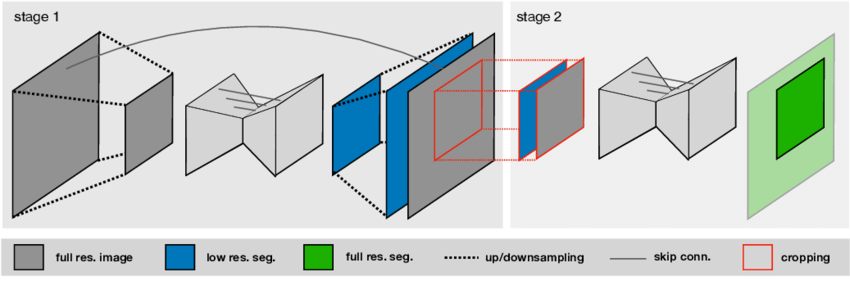
\includegraphics[width=1\linewidth]{images/UNet-Cascade}
	\caption{U-Net-Cascade\cite[4]{isensee_nnu-net_2018}}
	\label{fig:UNet-Cascade}
\end{figure}

\noindent\textbf{Stage 1}:\\
The process begins by downsampling the input images to a lower resolution. This reduction simplifies the image while retaining its core structural elements.
A standard U-Net then processes this low-resolution image, producing a segmentation that primarily captures the broader, global features.
While some detail is inevitably lost due to the reduced resolution,
this stage effectively provides an initial segmentation that identifies the general areas of interest within the scan.\\[1ex]
\noindent\textbf{Stage 2}:\\
The low-resolution segmentation from the first stage is then upscaled back to the original image size. This upscaled segmentation, capturing broad structures,
is concatenated with the original high-resolution scan, creating a guided version of the scan.
By merging the global information from the upscaled segmentation with the local detail of the original scan, a richer context is formed.
This guided scan is then cropped to focus on areas where the first stage identified potential regions of interest.
A standard U-Net then processes this cropped, guided scan, refining the segmentation further and honing in on the finer structures with greater precision.\\[1ex]
The U-Net cascade, in its essence, is a solution that seeks to balance the global and local context.
By starting with a bird's-eye view and then refining with granular detail, it aims to produce segmentations that capture intricate structures more accurately than a single-stage U-Net might.\\[1ex]
To tackle memory limitations, especially in settings with restricted computational capabilities, we can integrate this two-stage structure with the patch-wise U-Net.
Specifically, the second stage can be adapted to work on individual patches.
Although using this method might compromise some accuracy due to the limited context within each patch,
we anticipate that the first stage will provide sufficient contextual guidance to compensate. This adjustment allows the cascade to be more memory-efficient,
all while maintaining the advantages of a two-stage refinement. This revised cascade remains central to our study.

\chapter{Methodology}
In this work, we focused on a competitive analysis of three medical segmentation models with the objective of assessing the tradeoffs between performance, inference time and memory efficiency.
For the models, we focus on different variations of the U-Net architecture. The models employed for the training and evaluation include the use of normal $3$D U-Net, patch-wise U-Net,
patch-wise U-Net cascade. For a comparative analysis, we implemented them in PyTorch and trained them on some of the Medical Segmentation Decathlon (MSD) datasets.\\

\section{Data Collection and Preparation}
The first section of the methodology revolves around the selection and conditioning of datasets employed in model training and evaluation.
Recognizing the disparities among medical image segmentation tasks, we aimed for a broad evaluation by training our models on two datasets.
The Medical Segmentation Decathlon (MSD) offers ten distinct, task-specific datasets, which can be downloaded from \url{http://medicaldecathlon.com/}.
All the data was made available under the Creative Commons license CC-BY-SA $4.0$. This license allows us to use the data by citing this paper\cite[7]{simpson_large_2019}.

\newpage
\begin{table}[ht!]
\begin{center} {\footnotesize
\begin{tabular}{lccc}
\hline
	& \multicolumn{3}{c}{MSD Dataset}  \\
	& \multicolumn{1}{c}{size} & \multicolumn{1}{c}{shape} & \multicolumn{1}{c}{mean voxel count}\\
\hline
Task$01$\_BrainTumor & $484$ & $240\times240\times155$ & $8.928.000$ \\[1ex]
Task$02$\_Heart & $20$ & $320\times320\times90\mbox{-}130$ & $11.627.520$ \\[1ex]
Task$03$\_Liver & $131$ & $512\times512\times74\mbox{-}987$ & $117.340.457$ \\[1ex]
Task$04$\_Hippocampus & $260$ & $31\mbox{-}43\times40\mbox{-}59\times24\mbox{-}47$ & $62.793$ \\[1ex]
Task$05$\_Prostate & $32$ & $256\mbox{-}384\times256\mbox{-}384\times16\mbox{-}24$ & $1.924.224$ \\[1ex]
Task$06$\_Lung & $63$ & $512\times512\times112\mbox{-}636$ & $73.471.057$ \\[1ex]
Task$07$\_Pancreas & $281$ & $512\times512\times37\mbox{-}751$ & $24.926.070$ \\[1ex]
Task$08$\_HepaticVessel & $303$ & $512\times512\times24\mbox{-}181$ & $18.272.215$ \\[1ex]
Task$09$\_Spleen & $131$ & $512\times512\times31\mbox{-}168$ & $23.337.210$ \\[1ex]
Task$10$\_Colon & $126$ & $512\times512\times37\mbox{-}729$ & $28.057.730$ \\[1ex]
\hline
\end{tabular} }
\end{center}
\caption{\footnotesize This table shows the size, shape, and mean voxel count of each MSD dataset.
The shape is given as $\text{width}\times \text{height}\times \text{depth}$ when a dimension is variable, it is given as $\text{min}\mbox{-}\text{max}$.
The mean voxel count is calculated by taking the product of the width, height, and depth and then rounding the mean down to the next integer.}
\label{tab:msd}
\end{table}
\noindent While memory efficiency is a problem for images with a large voxel count, it is not so prominent for images with a low voxel count.
As our emphasis lay on addressing memory efficiency challenges associated with large voxel counts, we did not choose datasets with a low voxel count.
Since brain tumor segmentation is the most common dataset for medical image segmentation research, we picked the brain tumor dataset as our primary dataset.
To test the capabilities on datasets with a larger voxel count, we chose the liver dataset as our secondary dataset.\\[1ex]
\noindent To prepare our data for training, all image data undergoes normalization, and both images and labels are converted into $4$D tensors, adhering to the shape (channel, width, height, depth).
Notably, no form of data augmentation is applied. To ensure a rigorous model evaluation, we partition the datasets into three distinct subsets: training, validation, and testing.
The training subset is used for the actual training of the models, the validation subset assesses accuracy during the training phase and helps monitor how much the models are overfitting.
The testing subset is reserved for the ultimate model evaluation when the models are trained.
Specifically, we split the datasets  as follows: $60$\% for training, $20$\% for validation, and $20$\% for testing.

\section{Model Description}
Our investigation covers the following models: standard $3$D U-Net, patch-wise $3$D U-Net, and patch-wise $3$D U-Net cascade.

\subsection{3D U-Net}
Our choice of a foundational model is the standard $3$D U-Net, which has proven its prowess in a range of segmentation tasks.
At its inception, the model begins with a convolutional layer designed to generate $32$ channels. As data progresses deeper into the network, these channels expand in number,
marking the distinct stages of the descending U-Net structure, with output channels scaling at $64$, $128$, $256$, and finally culminating at $512$.\\[1ex]
While the quintessential U-Net relies on double convolutions at each of its stages, we sought improvements in this domain. To achieve this,
every stage in our U-Net is composed of two sequential convolution layers. Each convolution layer, characterized by a kernel size of $3$ and a padding of $1$,
is immediately followed by a Batch Normalization (BatchNorm) layer with a momentum of $0.1$ and a Rectified Linear Unit (ReLU) activation function.
This modified architecture is anticipated to lead to better training results and potentially better generalization\cite[7-8]{ioffe_batch_2015}.
The final output is then passed through a softmax activation function.\\[1ex]
Despite the advancements and the precision it offers, our $3$D U-Net reveals its Achilles heel when confronted with datasets boasting a hefty voxel count.
Its memory consumption makes it a formidable contender for standard GPUs, necessitating the use of high-tier graphics cards like the A$40$ or A$100$ to process such extensive datasets efficiently.

\subsection{Patch-wise U-Net}
Prioritizing GPU memory efficiency, the patch-wise U-Net presents a viable alternative. It maintains specifications consistent with the $3$D U-Net.
While there are multiple ways of patchifing a scan, we chose to just slice the scan in the last dimension every $16$ voxels, as this is easy to implement.
The patch-wise U-Net then segments these slices of height $16$ individually.
In instances where the image's last dimension isn't a multiple of $16$, the final patch undergoes zero-padding.
The produced patch segmentations are then reconstructed into a full segmentation.
These adaptations considerably diminish GPU memory consumption but also tend to compromise on accuracy because of the loss of global context.

\subsection{Patch-wise U-Net Cascade}
In contrast to the previously discussed U-Nets that produce segmentations at full resolution, the cascade approach follows a two-stage process:
initial segmentation at a reduced resolution, followed by a refinement at full resolution.\\[1ex]
\textbf{Stage 1}:
The input images are downscaled by a factor of $0.3$ for brain tumor and a factor of $0.2$ for the liver dataset, producing an image with reduced resolution. These downscaled images are then processed through a $3$D U-Net,
yielding a low-resolution segmentation.\\[1ex]
\textbf{Stage 2}:
The segmentation from the first stage is upscaled back to its original size and acts as guidance for the subsequent stage.
This upscaled segmentation is concatenated with the original image and then passed into a patch-wise U-Net in the second stage with the same specifications as the normal patch-wise U-Net.
Both stages can be trained independently of eatch other.\\

\noindent The key advantage of this cascade structure is memory efficiency. Both the patch-wise and the $3$D U-Net operating on downscaled images inherently require less memory.
This makes the cascade method more memory-efficient compared to the standard $3$D U-Net that operates at full resolution. Furthermore,
the low-resolution segmentation from the first stage is designed to compensate for the loss of spatial information, potentially enhancing the accuracy of the segmentation in the second stage.
As a result, the cascade U-Net is anticipated to deliver more accurate results than the standalone patch-wise U-Net.

\section{Environment and Tools}
All model training and evaluation were conducted using an NVIDIA A$40$ GPU with $48$GB of GPU memory. The experiments operated under a Linux Ubuntu $20.04$ amd$64$ environment. For the model's implementation,
we utilized the PyTorch framework.

\section{Training}
As the training process is a crucial component of our investigation, we elaborate on the training methodology in this section.
\subsection{Loss Function}
We employ Dice Loss for training the U-Nets. Witch is given by this formula, where TP is the number of true positives, FN is the number of false negatives, and FP is the number of false positives.
$$\mathcal{L}_{dice}=1-\frac{2*\text{TP}}{2*\text{TP}+\text{FN}+\text{FP}}$$
The loss is calculated for each channel, and then the mean is taken.
Given that our segmentations invariably incorporate a background channel, this channel is excluded from consideration.
The rationale behind this is that many images predominantly consist of background, and inclusion of this background could disproportionately dominate the loss calculation.
A potential pitfall emerges when the ground truth segmentation consists solely of the background. In such instances, the model only generates true negatives and false positives,
leading to a constant dice loss value of one, rendering gradient computation impossible. However, when training on entire images, this issue is circumvented, as all images contain non-background segmentations.
Conversely, for the patch-wise U-Net, where only sections of images serve as training data, instances may arise where the ground truth segmentation consists only of the background. To address this,
we ensure that the background channel is incorporated into the loss calculation for the patch-wise U-net and the second stage of the patch-wise U-Net cascade.

\subsection{Optimizer}
Across all experiments, we employ Adaptive Momentum Estimation (Adam)\cite{kingma_adam_2017} as our optimizer.
Instead of having a constant learning rate, Adam adjusts the learning rate at each iteration based on momentum,
which proves efficient in practice. For initialization, a learning rate of $3*10^{-4}$ is set.

\subsection{Epochs and Steps}
Since the datasets all vary in size, we chose a constant step count instead of a constant epoch count.
All models are trained on $90.000$ steps. This proved to be enough for training the models.
We made checkpoints after each epoch and chose the checkpoint with the best validation accuracy as the final model.

\section{Evaluation Metrics}
Upon completion of the training phase, the models are evaluated based on three pivotal metrics: accuracy, inference time, and GPU memory consumption during inference.
Each model is subject to inference on the test datasets for $2000$ steps, and the arithmetic mean for each metric is then computed.

\subsection{Accuracy}
We gauge accuracy by computing the dice loss on the complete segmentations. Meaning that for the patch-wise and patch-wise U-Net cascade,
we reconstruct the whole segmentation from the patches before calculating the loss. Given that none of the segmentations is solely composed of background,
we exclude the background channel in our calculations, as elaborated in Section $2.4.1$. Instead of taking the mean of all channel losses, we monitor the dice losses for each channel individually.

\subsection{GPU Memory Monitoring}
To determine GPU memory efficiency, we could record the GPU memory allocation immediately post-inference, when both the model and data persist on the GPU.
Since we are only interested in the maximum memory consumption, this could give false values that are too low if the model uses more memory during the inference that is then freed post-inference.
Conveniently, PyTorch offers a function that returns the maximum memory allocation for the whole run. This function is called once after all steps of inference are completed and the maximum value is recorded.

\subsection{Inference Time}
An accurate representation of model efficiency also mandates the measurement of inference time, the duration a model requires to annotate a single image.
The stopwatch is activated the moment an image is fed into the model and halted once the output is generated. For the patch-wise U-Net and patch-wise U-Net cascade,
the metric also encapsulates the time consumed to reconstruct the whole segmentation.

\chapter{Implementation}
In this chapter, we elaborate on the implementation, which can be found on \href{https://github.com/janiswehen/hpi-ml-ba}{GitHub}. Our project primarily utilizes the PyTorch framework due to its flexibility and widespread adoption in the deep learning community.
\section{Model}
Our foundational architecture was the $3$D U-Net. Interestingly, a single \code{UNet3d} class was developed to represent all three U-Net variations. The uniqueness of each U-Net type does not emerge in the architectural structure,
but rather in their distinct training and inference implementation.
\section{Dataset Loading with MSDDataset}
To streamline data handling, the \code{MSDDataset} class was established. This class serves the pivotal role of loading and preprocessing the MSD datasets.
One of its primary functions is to interpret the \code{dataset.json} file inherent to every MSD dataset. This JSON file delineates dataset attributes such as its type, the labels of input and output channels,
and the directory paths to the respective images and labels. Upon these directives, the \code{MSDDataset} class proceeds to load, normalize, and prepare the datasets for subsequent stages.\\
To facilitate diverse data transformation requirements, we introduced a suite of wrapper datasets:
\begin{enumerate}
	\item \code{DownsampledDataset}: This wrapper engages PyTorch's Upsample class to downscale both images and labels. An inherent rescaling function allows it to restore the datasets to their native resolutions when needed.
	\item \code{SlicedDataset}: This dataset wrapper slices the image and label into patches of the same size, padding the last patch if needed. A reconstruction function is embedded for scenarios necessitating a reversion to the original dataset dimensions.
    \item \code{CombinedDataset}: This is a hybrid class that amalgamates two datasets. While it offers customizable combination functions,
	its default behavior is to concatenate the first dataset's image with the second dataset's label, thereby formulating a guided image. The label of the first dataset is kept.
\end{enumerate}

\section{Training Framework}
For the training, we implemented four trainer classes. Each training setup uses data loaders for efficient asynchronous data loading.
The type of dataset and model requirements dictate our choice of data loader and associated wrappers. Here's a breakdown:

\begin{enumerate}
	\item \code{FullUnetTrainer}: For the standard $3$D U-Net, we mainly use the \code{MSDDataset} class. It allows us to go through the entire dataset, one epoch at a time.
	\item \code{PatchUnetTrainer}: For this version, we use the \code{MSDDataset} class wrapped within the \code{SlicedDataset}. This setup divides the data into patches.
	In each step backpropagation is done on all patches of the current image indevidualy.
	\item \code{CascadeStage1UnetTrainer}: The first stage is trained using the \code{MSDDataset} class inside the \code{DownsampledDataset} wrapper. This wrapper initially downscales the dataset to fit the requirements of this stage.
	\item \code{CascadeStage2UnetTrainer}: The process for this stage involves several steps:
	\begin{enumerate}
		\item Start by wrapping the \code{MSDDataset} in the  \code{DownsampledDataset} wrapper, setting it to downscale, and then rescale the image and label.
        \item Next, the \code{CombinedDataset} wrapper merges the rescaled label with the original image, providing the new input. The original label is kept as the ground truth.
		\item This combined dataset is then wrapped with the \code{SlicedDataset} to train the model on guided patches, similar to the patch-wise U-Net approach.
	\end{enumerate}
\end{enumerate}

\noindent The model's training can be started using a dedicated script that accepts configuration files as input. These files are amalgamated into a comprehensive configuration dictionary,
which in turn drives the initialization of the apt training class.\\[1ex]
\section{Model Evaluation}
The model can be evaluated using three different evaluator classes. Each evaluator class uses a data loader to load the data. For the cascade,
the two stages are connected to evaluate the performance of the entire cascade. Every result during training and evaluation is then logged using Weights and Biases.

\chapter{Experimental Results}

In our journey to improve and adapt the U-Net architecture, it's crucial to see how well our changes work in practice. In this chapter,
we present the results garnered from our experiments, which provide a clear picture of the advantages, trade-offs, and potential areas of improvement associated with our implementations.

\section{Brain Tumor Dataset}
The first dataset we trained our models on was the brain tumor dataset.

\begin{table}[ht!]
\begin{center} {\footnotesize
\begin{tabular}{lccc}
\hline
	& \multicolumn{3}{c}{Brain Tumor Dataset accuracy} \\
	& \multicolumn{1}{c}{edema} & \multicolumn{1}{c}{non-enhancing tumor} & \multicolumn{1}{c}{enhancing tumor}\\
\hline
$3$D U-Net & $\mathbf{80.13}$ & $\mathbf{60.80}$ & $\mathbf{75.99}$ \\[1ex]
patch-wise U-Net & $70.01$ & $31.02$ & $55.58$ \\[1ex]
patch-wise U-Net cascade & $77.54$ & $56.84$ & $71.18$ \\[1ex]
\hline
\end{tabular} }
\end{center}
\caption{\footnotesize This table shows the mean dice scores for the test split of the brain tumor dataset. The best scores are highlighted in bold.}
\label{tab:bt-accuracy}
\end{table}

\noindent The $3$D U-Net demonstrates superior performance in all metrics. While the patch-wise U-Net has the least impressive results across categories, the patch-wise U-Net cascade fares better.
Notably, it surpasses the patch-wise U-Net considerably and even approaches the 3D U-Net's precision.
Inspecting the results, we notice that all models struggle to segment more fine structures, like the non-enhancing tumor.\newpage

\begin{table}[ht!]
\begin{center} {\footnotesize
\begin{tabular}{lccc}
\hline
	& \multicolumn{2}{c}{Brain Tumor Dataset efficiency} \\
	& \multicolumn{1}{c}{GPU memory(GB)} & \multicolumn{1}{c}{inference time(s)} \\
\hline
$3$D U-Net & $21.5$ & $\mathbf{0.35}$ \\[1ex]
patch-wise U-Net & $2.9$ & $0.67$ \\[1ex]
patch-wise U-Net cascade & $\mathbf{2.8}$ & $0.91$\\[1ex]
\hline
\end{tabular} }
\end{center}
\caption{\footnotesize This table shows the mean inference time for the test split of the brain tumor dataset in seconds and the maximum GPU memory consumption in GB.
The best scores are highlighted in bold.}
\label{tab:bt-efficiency}
\end{table}

\noindent The standard $3$D U-Net is the most demanding in terms of GPU memory. Intriguingly, the patch-wise U-Net cascade consumes less memory than its standard counterpart,
even though it inherently incorporates the patch-wise U-Net. In terms of inference time, the $3$D U-Net shines the brightest, whereas the cascade model lags behind the standard patch-wise model, probably due to its two-stage processing.

\section{Liver Dataset}
Let us now take a look at the results for the liver dataset. Here, we encountered some problems. The $3$D U-Net was unable to train on the liver dataset due to the large voxel count.
The training process would run out of memory when the model tried to allocate $325$ GB of GPU memory.
The patch-wise U-Net, though trainable, initially produced only background segmentations.
We pinpointed the inclusion of the background channel in the loss calculation as the culprit. The inclusion of the background channel dominated the loss, so it was beneficial for the model to only segment the background. By excluding this channel,
the model's training performance improved significantly. Since this produces a constant loss when the patches consist of only background, we skipped these empty patches during the training process.

\newpage
\begin{table}[ht!]
\begin{center} {\footnotesize
\begin{tabular}{lccc}
\hline
	& \multicolumn{2}{c}{Liver Dataset accuracy} \\
	& \multicolumn{1}{c}{liver} & \multicolumn{1}{c}{cancer} \\
\hline
$3$D U-Net & $-$ & $-$ \\[1ex]
patch-wise U-Net & $87.01$ & $22.22$ \\[1ex]
patch-wise U-Net cascade & $\mathbf{92.00}$ & $\mathbf{25.05}$ \\[1ex]
\hline
\end{tabular} }
\end{center}
\caption{\footnotesize This table shows the mean dice scores for the test split of the liver dataset. The best scores are highlighted in bold.}
\label{tab:l-accuracy}
\end{table}

\noindent The patch-wise U-Net cascade claims the top spot for performance on the liver dataset. The $3$D U-Net, on the other hand, was unable to produce any results due to the extensive voxel count.
When focusing on segmenting cancer, the models showed room for improvement. However, liver segmentation showed promising results.

\begin{table}[ht!]
\begin{center} {\footnotesize
\begin{tabular}{lccc}
\hline
	& \multicolumn{2}{c}{Liver Dataset efficiency} \\
	& \multicolumn{1}{c}{GPU memory(GB)} & \multicolumn{1}{c}{inference time(s)} \\
\hline
$3$D U-Net & $\geq325$ & $-$ \\[1ex]
patch-wise U-Net & $\mathbf{10.6}$ & $\mathbf{4.49}$ \\[1ex]
patch-wise U-Net cascade & $12.4$ & $5.90$\\[1ex]
\hline
\end{tabular} }
\end{center}
\caption{\footnotesize This table shows the mean inference time for the test split of the liver dataset in seconds and the maximum GPU memory consumption in GB. The best scores are highlighted in bold.}
\label{tab:l-efficiency}
\end{table}

\noindent Given the $3$D U-Net's memory requirements,
this model isn't a feasible choice even for high-end GPUs like the A$100$. Implementing it across multiple GPUs might be a solution, but it brings its own set of challenges.
Conversely, both patch-wise models prove to be adaptable choices for conventional GPUs with $16$ GB or more memory. Unlike for inference on the brain tumor dataset,
the patch-wise U-Net cascade takes up more memory than the patch-wise U-Net. Similar to the brain tumor dataset, the patch-wise U-Net is faster than the patch-wise U-Net cascade.

\chapter{Discussion}
In this section, we dive into the implications of our experimental findings, addressing both the strengths and constraints of our study, along with potential avenues for further refinement.

\section{Conclusion}
Our results from the brain tumor dataset indicate that the $3$D U-Net stands out in terms of accuracy. However, this prowess is accompanied by increased GPU memory demands.
This isn't an issue for datasets with moderate voxel counts, such as the brain tumor dataset, but it emerges as a constraint for voluminous datasets like the liver dataset.\\[1ex]
The output size of a convolutional layer roughly scales linearly with the number of input voxels. Since the U-Net architecture mostly consists of convolutional layers, we assume that the GPU memory consumption also roughly scales linearly with voxel count.
This would mean that the ratio between GPU memory consumption and voxel count is roughly constant.
This allows us to make an educated guess for how much GPU memory a normal U-Net would allocate for an image with a given voxel count using the following formula where $M_v$ is the GPU memory consumption for a voxel count of $v$
$$\frac{M_{v_1}}{v_1}\approx\frac{M_{v_2}}{v_2}.$$
Rearranging this formula and using the data on memory consumption we got for the brain tumor dataset, we can approximate the memory consumption of an average-sized scan from the liver dataset.
From the formula, we would necessitate an average memory allocation of approximately $\frac{21,5~\text{GB} * 117.340.457}{8.928.000}\approx282~\text{GB}$.
For the initial scan of size $512\times512\times771$ from the liver dataset, which was the one where the training halted because it attempted to allocate $325$ GB, we get an estimated memory demand of $\frac{21,5~\text{GB} * 512*512*771}{8.928.000}\approx486~\text{GB}$.
This far exceeds the capacity of a single GPU.
To illustrate, NVIDIA's A$100$ offers a peak memory of $100~\text{GB}$, and even this premium GPU falls short. Addressing this would necessitate employing multiple GPUs,
bringing the added complexity of multi-GPU support.\\[1ex]
Our findings posit the patch-wise U-Net and its cascade counterpart as promising alternatives if one allows some loss of accuracy.
Notably, the cascade variant has a longer inference time than the normal patch-wise U-Net and is more complex to train since one has to train two networks. However, this cascade structure elevates the accuracy of the model by far, making it compatible with the normal U-Net.
When pitted against the cascade, the sole advantages of the standard patch-wise U-Net are its swifter inference times and simpler implementation. Given these trade-offs, we advocate for the patch-wise U-Net cascade over its simpler counterpart in most scenarios.\\[1ex]
For datasets comprising low-resolution images, the original $3$D U-Net remains the gold standard due to its superior speed and accuracy.
Yet, when tackling high-resolution imagery, the normal U-Net is not feasible, and we have to rely on models that compromise on efficiency to reduce the memory demand.

\section{Potential Improvements}
While our models have demonstrated potential, there remains a significant gap between our results and the benchmarks set by contemporary studies.
For context, in the nnU-Net paper, competitors in the MSD achieved a dice score of $73.71$ for cancer detection in the liver dataset\cite[9]{isensee_nnu-net_2018}.
When juxtaposed with our dice score of $25.05$ for the same task, the disparity is evident: our models are not yet on par with the best in the field.
Several strategies could bridge this gap:
\begin{enumerate}
	\item \textbf{Data Augmentation}: Introducing variations in the training data through techniques like rotation, scaling, and flipping can make our model more robust and potentially improve its generalization capability.
	\item \textbf{Focusing on the Region of Interest}: In the preprocessing phase, cropping images to highlight the region of interest can ensure the model's training focuses more intently on the salient data, potentially improving accuracy.
	\item \textbf{Leveraging Pre-training}: Training our model on diverse datasets before fine-tuning it on the specific dataset of interest can provide a more generalized feature representation,
	which might boost performance when the model is subsequently fine-tuned. Unsupervised learning techniques could also be employed to generate a more robust feature representation.
\end{enumerate}
By integrating these strategies, we believe we will be able to enhance our model's performance and bring it closer to state-of-the-art benchmarks in future iterations.

\section{Future Work}
Other interesting further investigations could be to compare the patch-wise U-Net cascade to other models that try to address the memory efficiency problem.
One other worthy contestant that could be a memory-efficient alternative to the $3$D U-Net is the patch-free segmentation model proposed in this paper\cite{wang_super-resolution_2023}.\\[1ex]
It would also be interesting to combine the patch-wise U-Net cascade with other memory reduction techniques such as model pruning, quantization, or memory-efficient backpropagation.
